\chapter{Att bygga ett system i ROS}
\chapterprecis{\LARGE{---- Martin Lundberg ----}}
\label{cha:indiv-report-lundberg}

\section{Inledning}
\label{sec:introduction-lundberg}

I ROS finns det många verktyg för att bygga upp ett system. ROS gör det enkelt att köra fler processer och kommunicera mellan dessa. Det hjälper även till att tydliggöra uppdelningar av ett program i separata moduler som enkelt kan återanvändas och vidareutvecklas separat utan att påverka de övriga modulerna.


\subsection{Syfte}
\label{sec:purpose-lundberg}

Syftet med den här rapporten är att utforska olika metoder i ROS för att bygga upp ett system. Rapporten ska även jämföra lösningarna i ROS med andra metoder för att ge fler perspektiv på hur ett system kan byggas upp. 

\subsection{Frågeställning}
\label{sec:issue-lundberg}

Följande frågeställningar ska behandlas och besvaras i denna rapport.

\begin{enumerate}
	\item Hur kan en arkitektur implementeras i ROS?
	
	\item Hur påverkade valet att använda ROS uppbyggnaden av systemet?
\end{enumerate}


\section{Bakgrund}
\label{sec:background-lundberg}

\begin{comment}
	ROS från vårt perspektiv, varför vi använde ROS, sammanhanget för rapporten
\end{comment}

I det projekt som utvecklats och beskrivits i huvuddelen av denna rapport användes ROS redan från ett tidigt skede. En anledning till att just ROS valdes var för att projektets kund hade det som önskemål, dock såg projektmedlemmarna tidigt att ROS förde med sig många fördelar. Användningen av ROS planerades redan i arkitekturen som är utformad helt med förutsättningen att ROS skulle användas för implementationen.

I denna rapport utreds hur ROS kan användas i implementationen av en arkitektur. Arkitekturen hade som mål att vara så modulär som möjligt då det skulle underlätta för projektets kund som vill kunna vidareutveckla olika delar av systemet i framtiden.

I ett sent skede i projektet behövde stora ändringar göras i arkitekturen vilket gjorde att ROS uteslöts helt. Detta gav ytterligare ett perspektiv att utgå från i den här utredningen.


\section{Teori}
\label{sec:theory-lundberg}

\subsection{ROS}
ROS står för Robot Operating System men är inte ett fullt operativsystem i den traditionella meningen. Istället är det ett system som körs i ett vanligt operativsystem och som ger användaren möjlighet att på ett enkelt sätt köra fler processer och kommunicera mellan dessa \cite{quigley2009ros}. En process som körs i ROS kallas för en nod och ROS tillhandahåller verktyg för att styra dessa noder. Det är ofta en bra tumregel att tänka att en nod motsvarar en modul i arkitekturen, men en modul skulle även kunna bestå av ett flertal noder.

ROS har även verktyg för att på ett enkelt och strukturerat sätt kommunicera mellan noder genom meddelanden (eng. messages). Dessa meddelanden är strikt typade och kan skickas mellan noder på två olika sätt:

\begin{enumerate}
	\item Genom att en nod publicerar på en namngiven kanal (eng. topic) som en annan nod kan lyssna på.
	
	\item En nod kan tillhandahålla en service som en annan nod kan kalla på för att utföra något arbete och få tillbaka resultatet i form av ett meddelande.
\end{enumerate}

Den här rapporten ska utforska hur dessa verktyg kan användas för att bygga upp ett system.

\subsection{Pipe and filter-modellen}
En välkänd modell för att bygga upp mjukvarusystem är pipe and filter-modellen. Den beskrivs av Garlan och Shaw \cite{garlan1993introduction} som en modell där varje komponent i systemet har bestämda indata och utdata. Komponenterna behandlar indatan och producerar utdata som kan skickas vidare till nästa steg i modellen.

I en traditionell pipe and filter-modell behandlas indatan kontinuerligt så att utdata produceras innan hela strömmen av indata har nått fram, därav namnet filter. I detta projekt användes dock ett specialfall av modellen där varje komponent kräver ett helt block av indata som sedan behandlas för att producera ett block av utdata. Det ska noteras att trots att varje modul endast tar kompletta block av indata snarare än strömmar så kan modulerna internt arbeta med strömmar av data och inkrementellt bygga upp resultatet.


\section{Metod}
\label{sec:method-lundberg}
I detta kapitel beskrivs metoden som användes för att ta fram systemets arkitektur och hur beslut fattades om systemets uppbyggnad.

\subsection{Arkitekturens framtagande}
Arkitekturen för systemet har tagits fram med en iterativ process. Det första steget var att tänka igenom olika use cases för systemet och utifrån det ta fram de funktioner som programvaran måste innehålla. Detta resulterade i en systemanatomi som användes i det kommande arbetet.

Nästa steg var att se vilka funktioner som var relaterade till varandra och bestämma vilka noder systemet skulle bestå av och även hur dessa skulle kommunicera med varandra. Det var tydligt att programmets funktionalitet kunde delas upp i tre distinkta moduler:

\begin{enumerate}
	\item punktmolnshantering
	
	\item meshgenerering
	
	\item hantering av 3D-skrivare.
\end{enumerate}

Utöver de delarna behövdes även ett sätt att styra processen. För detta ändamål infördes ett grafiskt användargränssnitt och även ett kommandoradsgränssnitt som skulle kunna initiera hela eller delar av processen.

Då projektet byggde vidare på ett system kallat TreeD från förra året för att styra hårdvaran behövde även det tidigare systemet tas i åtanke när arkitekturen togs fram. Fler alternativ för att kommunicera med det tidigare systemet utforskades men i slutändan beslutades det att en egen nod skulle kalla på det tidigare systemets kommandoradsgränssnitt för att på så vis slippa sätta sig in i tidigare kod för att lista ut vilka funktioner som behövde kallas.

Ett viktigt mål med arkitekturen var att systemet skulle vara modulärt. Tidigt i arbetet bestämdes det att en variant av pipe and filter-modellen skulle vara lämplig. Där skickas resultatet från ett steg vidare som indata till nästa steg. En stor fördel med denna modell är att den gör det möjligt att byta ut enskilda delar utan att göra om hela systemet \cite{garlan1993introduction}. Detta är något som uppfyller de krav på moduläritet och underhållbarhet som ställdes på systemet.

\subsection{Systemet i ROS}
För att bygga systemet i ROS togs ett första förslag på en arkitektur fram där de moduler som beskrevs ovan motsvarade en varsin ROS-nod. För att kommunicera med varandra skulle noderna använda sig av topics för att ta emot kommandon och skicka resultatet av utförda beräkningar. Att använda topics hade fördelen att det är ett enkelt och snabbt sätt att komma igång med kommunikation mellan noder. Det var dock ett naivt sätt att implementera systemet i det här fallet då en topic-baserad lösning gör väldigt lite för att upprätthålla den tänkta arkitekturen. Eftersom vilken nod som helst kan lyssna på en topic blir det svårare att se kommunikationsvägarna mellan olika noder och därför blir det även svårare för en utomstående att förstå systemets uppbyggnad och vidareutveckla systemet.

För att göra systemet tydligare togs en ny arkitektur fram som istället var baserad på service-anrop. I denna arkitektur tillhandahåller modulerna en service som en annan nod kan kalla på för att utföra ett specifikt arbete. När arbetet är utfört returneras resultatet till noden som utförde service-anropet. Detta system gör det mycket tydligare vad de olika noderna gör och hur de kommunicerar med varandra och det är den slutgiltiga arkitekturen i ROS som togs fram för projektet.

\subsection{Systemet utan ROS}
Då projektets förutsättningar ändrades långt in i utvecklingsfasen behövde en ny arkitektur tas fram. Den nya arkitekturen behövde inte kommunicera med hårdvaran på något sätt utan skulle endast läsa in punktmoln från filer på disk. För att underlätta utvecklingsarbetet och för att det inte längre var lika aktuellt att använda ROS bestämdes det att den nya arkitekturen inte skulle vara baserad på ROS. Systemets uppbyggnad på modulnivå behölls dock så lik den tidigare arkitekturen som möjligt där den största skillnaden är att någon koppling till TreeD inte längre finns.

För att göra det fortsatta arbetet så enkelt som möjligt då det var begränsat med tid kvar beslutades det att systemet skulle byggas upp med klasser i C++, där varje modul motsvarar en klass som tillhandahåller modulens funktionalitet.

\subsection{Dokumentering av processen}
Under framtagandet av arkitekturen dokumenterades arbetet kontinuerligt i form av mötesprotokoll och diverse skisser och blockscheman som togs fram. Stora delar av arbetet med arkitekturen finns dokumenterat i projektets arkitekturbeskrivning där alla beslut som tagits om arkitekturen finns. Den innehåller även motiveringar till de beslut som fattats och, i relevanta fall, alternativa lösningar som diskuterades men som inte kom med i den slutgiltiga arkitekturen. Denna dokumentation används som underlag för att kunna svarar på frågeställningarna i denna rapport.


\section{Resultat}
\label{sec:results-lundberg}

Sent i projektet stötte gruppen på problem som inte gick att lösa inom en rimlig tidsram. Därför behövde projektets mål omdefinieras och på grund av det togs även ny arkitektur fram, denna gång utan ROS. I detta avsnitt visas båda de arkitekturer som togs fram för projektet.

\subsection{Arkitekturen i ROS}
Den ROS-baserade arkitektur som togs fram för projektet visas i figur \ref{fig:arkitektur}. Varje block i figuren motsvarar en nod i ROS och kommunikationsvägarna mellan noderna illustreras med pilar. All kommunikation mellan noderna utförs i form av service-anrop i ROS.

\begin{figure}[h]
	\centering
	\includegraphics[width=15cm]{figures/arkitektur.png}
	\caption{Systemets arkitektur i ROS.}
	\label{fig:arkitektur}
\end{figure}

Tidigt i projektet togs ett annat förslag på en arkitektur fram i ROS som är väsentligen samma som den i figur \ref{fig:arkitektur} men med den enda skillnaden att kommunikationen skulle skötas via topics istället för service-anrop. Detta skulle innebära att en egen topic skapades för varje kommunikationsväg som visas i figuren. 

Detta arkitekturförslag är också intressant för denna rapport då det visar på en del skillnader mellan olika sätt att 

\subsection{Arkitekturen utan ROS}
Den nya arkitekturen som togs fram utan ROS är uppbyggd enligt samma modell i grunden. Dock är den skriven helt i C++ och uppbyggd med hjälp av klasser som tillhandahåller den funktionalitet som tidigare låg i ROS-noder. Den nya arkitekturen använder inte heller det tidigare projektet TreeD så wrappern för den mjukvaran är borttagen. I detta system läses punktmolnsfiler in av klienten som sedan använder funktionaliteten i klasserna för att behandla punktmolnen. Klassindelningen och kopplingen mellan dem beskrivs i figur \ref{fig:klasser}.

\begin{figure}[h]
	\centering
	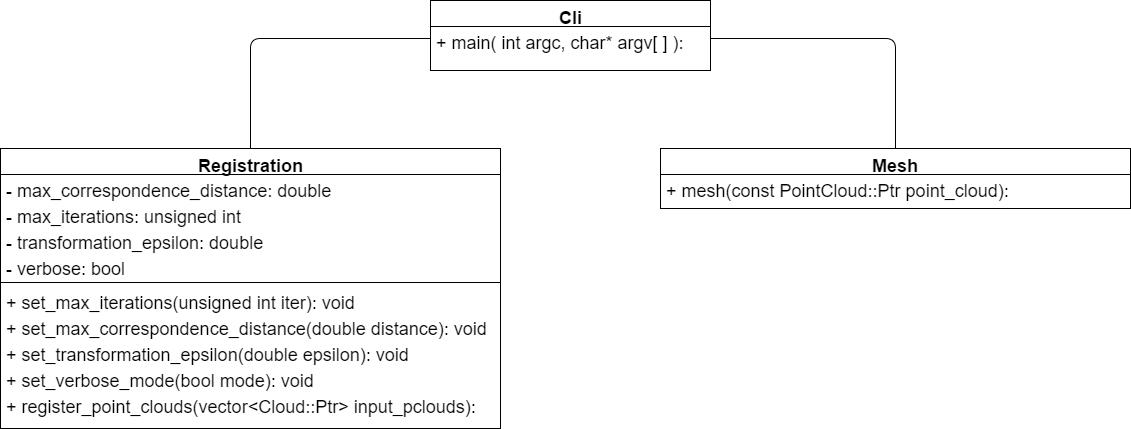
\includegraphics[width=15cm]{figures/klassdiagram.png}
	\caption{Systemets arkitektur utan ROS.}
	\label{fig:klasser}
\end{figure}


\section{Diskussion}
\label{sec:discussion-lundberg}

Resultatet av arbetet var två olika arkitekturer och implementationer av i grunden samma arkitekturidé. Detta ger möjlighet att jämföra ett system byggt i ROS med i grunden samma system byggt utan ROS.

Under arbetet med att ta fram och implementera dessa arkitekturer framkom en del för- och nackdelar med båda alternativen. Dessa diskuteras i detta avsnitt.

Det ROS-baserade systemet implementerades med service-anrop som beskrevs i avsnitt \ref{sec:results-lundberg}. Detta sätt att kommunicera gör det tydligt hur en nod kommunicerar med andra noder och hur systemet hänger ihop. Det undviker även så kallad spaghettikod där olika data och funktionsanrop skickas runt lite hur som helst utan någon tydlig struktur, vilket gör koden väldigt svår att förstå och underhålla. Dock märktes det senare under utvecklingsarbetet att det gjorde systemet stelt och det resulterade i mycket mer arbete för att till exempel kunna kommunicera delresultat från en nod som tar väldigt lång tid att köra. För att kunna se delresultat från en nod som körs genom ett service-anrop skulle noden behöva publicera delresultaten på en topic som en annan nod kan lyssna på. Detta gör dock att systemets modell bryts vilket gör att många av de fördelar som finns med att använda service-anrop går förlorade.

Det klassbaserade systemet däremot har mer flexibilitet i hur det implementeras. Det krävs dock lite tanke för att bibehålla moduläriteten i en sådan implementation.

\subsection{Portabilitet}
En viktig fördel med ROS är då man vill använda systemet tillsammans med andra ROS-baserade system. Eftersom kommunikation inom ROS är tydligt definierad kan man skriva en egen ROS-nod som använder sig av andra existerande noder och på så vis enkelt använda existerande system. Det kräver dock att det existerande systemet antingen är utförligt dokumenterat eller har en så pass tydlig struktur att det går att förstå hur man ska kommunicera med olika noder.

Den klassbaserade implementationen kan dock ses som mer portabel då den inte ska integreras med andra ROS-system. Klasserna som systemet är uppbyggt av kan importeras och användas i ett annat projekt oavsett om det använder ROS eller inte.

\subsection{Att gå från ROS till klasser}
En stor fördel med att systemet byggts upp så modulärt redan från början var att det var relativt smärtfritt att gå från den ROS-baserade arkitekturen till den klassbaserade. Mycket av den kod som hade skrivits kunde återanvändas och det var inga problem att implementera i grunden samma arkitektur både med och utan ROS.

Om det ROS-baserade systemet istället hade implementerats med kommunikation genom topics hade det varit svårare att separera modulerna och bryta ut funktionaliteten då modulerna hade haft en högre grad av koppling mellan sig. All kommunikation i det ROS-baserade systemet sköttes via service-anrop vilka kan liknas väldigt mycket vid klassiska funktionsanrop där någon indata ges och något resultat returneras när funktionen är klar. Detta gjorde det relativt enkelt att gå från ROS-systemet till det klassbaserade systemet.

\subsection{Hållbarhet}
Då olika ROS-noder körs som olika processer i operativsystemet och därför kan köras parallellt har ett ROS-baserat system en teoretisk möjlighet att vara mer energieffektivt än det klassbaserade system som implementerades i projektet (detta under förutsättning att stora beräkningar inte parallelliseras genom exempelvis flertrådad körning). I detta projekt skulle det dock ha minimal inverkan då varje större steg i processen var beroende av resultatet i det tidigare steget och modulerna kunde därför väldigt sällan köras parallellt.


\section{Slutsatser}
\label{sec:conclusions-lundberg}

Ett ROS-system byggt helt på service-anrop ger god separation mellan noderna och definierar tydligt hur kommunikation ska ske. Det förhindrar även att snabba fullösningar implementeras där data skickas utanför den fastställda strukturen för att underlätta utvecklingen på kort sikt men göra systemet svårare att underhålla på lång sikt. Ett service-baserad system är dock stelt och det är svårt att lägga till ytterligare kommunikationsvägar i efterhand. Det är därför tydligt att en balans mellan service- och topic-baserade system måste hittas då ett system designas. 


\begin{comment}
- Återkoppling till frågeställningar
– Nåddes syftet?
– Viktigaste lärdomar

Fördel med modulär arkitektur, gick att byta implementation enkelt och återanvända mycket kod

Viktigt att dokumentera arkitektur för underhåll, vidareutveckling


Hur kan en arkitektur implementeras i ROS?
Hur påverkade valet att använda ROS uppbyggnaden av systemet?
\end{comment}

%%%%%%%%%%%%%%%%%%%%%%%%%%%%%%%%%%%%%%%%%%%%%%%%%%%%%%%%%%%%%%%%%%%%%%
%%% person-report.tex ends here
